\documentclass[table]{beamer}

% Customize slide appearance
\mode<presentation>
{
  \usetheme{Warsaw}
  \setbeamercovered{transparent}
}


\usepackage[english]{babel}
\usepackage{times}
\usefonttheme[onlymath]{serif} 
\setbeamertemplate{navigation symbols}{}

% You can add any graphics to every slide by following command:
% \logo{\resizebox{0.1\textwidth}{!}{\includegraphics{col_small}}}
% \logo{\resizebox{0.2\textwidth}{!}{\includegraphics{imperialblue}}}

% Uncomment this, if you want the table of contents before each subsection.
% However, to edit slides in TeXWord avoiding this feature is good idea.
% \AtBeginSubsection[]
% {
%   \begin{frame}<beamer>
%     \frametitle{Outline}
%     \tableofcontents[currentsection,currentsubsection]
%   \end{frame}
% }

% If you wish to uncover everything in a step-wise fashion, uncomment
% the following command: 
%\beamerdefaultoverlayspecification{<+->}
\xdefinecolor{keyword}{rgb}{0,0,1}
\xdefinecolor{ctext}{rgb}{0.64,0.08,0.08}
\xdefinecolor{cline}{rgb}{0.17,0.57,0.69}
\xdefinecolor{comment}{rgb}{0,0.5,0.0}
\newif\ifschigh\schighfalse
\newcommand{\kw}[1]{\ifschigh\textcolor{red}{#1}\else\textcolor{keyword}{#1}\fi}
\newcommand{\kt}[1]{\ifschigh\textcolor{red}{#1}\else\textcolor{ctext}{#1}\fi}
\newcommand{\kc}[1]{\ifschigh\textcolor{red}{#1}\else\textcolor{comment}{#1}\fi}
\addtobeamertemplate{alerted text begin}{\global\schightrue%
}{}
\defbeamertemplate*{alerted text end}{default}{\global\schighfalse%
}



\newcounter{sckll}
\newcommand{\kr}{\setcounter{sckll}{1}}
\newcommand{\krr}[1]{\setcounter{sckll}{#1}}
\newcommand{\klvalue}{\ifnum\value{sckll}<10{\hphantom{0}}\fi\arabic{sckll}\addtocounter{sckll}{1}}
\newcommand{\kl}{\ifschigh\textcolor{red}{\klvalue}\else\textcolor{cline}{\klvalue}\fi\hspace{2ex}}
\newif\ifhandout
\handouttrue
\mode<beamer>{\handoutfalse}

\let\oldurl=\url
\renewcommand{\url}[1]{\textcolor{blue}{\oldurl{#1}}}

\usepackage{tikz, pgfbaseplot, pgflibrarysnakes,pgflibraryarrows}

\begin{document}

% Title Data. We keep it after \begin{document} 
% to enable editing text in BaKoMa TeX Word.

\title[C for Science - Lecture 1]{Computing in C for Science}
\subtitle{Lecture 1 of 5}

% Use the \inst command to identify several affiliations.
\author[Steven Capper]{Dr. Steven Capper \\ \url{http://www2.imperial.ac.uk/~sdc99/ccourse/}
{\tt steven.capper99@imperial.ac.uk}}

\date{$16^\text{th}$ November 2011 }

\subject{C for Science} % Should be passed to PDF [YNI]
{
\logo{\includegraphics[width=0.30\textwidth]{imperialblue}}
\begin{frame}
  \titlepage
\end{frame}
}

%\section{Introduction}
%\subsection{Introduction to the Course}

\begin{frame}
\frametitle{Introduction to the Course}
This course is based on the C course written by my PhD supervisor Dan Moore:
\url{http://www.ma.ic.ac.uk/~drmii}
\begin{block}<+->{Aims of the Course}
\begin{itemize}
\item To introduce modern C programming from scratch and,
\item provide insight into scientific computing (floating point arithmetic, optimisation, $\ldots$).
\end{itemize}
\end{block}

\begin{block}<+->{Five lectures spread over five weeks.}
\begin{itemize}
\item Each lecture will take $\approx 1$ hour,
\item and involve at least an hour of practical work.
\item This is very intense.
\item Please feel free to ask questions outside course hours.
\end{itemize}
\end{block}
\end{frame}

%\subsection{History and Motivation}
\begin{frame}
\frametitle{A Rough History of C}
\begin{block}<+->{Invented $\approx1970$}
By Dennis Ritchie working in Bell Labs USA; to facilitate development of
a portable UNIX.
\end{block}
\begin{block}<+->{C has been standardised}
\begin{itemize}
\item 1989 ANSI standard ratified \emph{ANS X3.159-1989}.
\alert{\item 1990 ISO standard \emph{ISO/IEC 9899:1990}. Aka \emph{C90}.}
\item 2000 ISO standard \emph{ISO/IEC 9899:1999}. Aka \emph{C99}.
\end{itemize}
\end{block}
\begin{block}<+->{C has evolved into C++}
Bjarne Stroustrup developed C++ (C with class). Unlike C, C++ is still under
very active development (C++11 being the most recent standard at the time of
writing).
\end{block}
\end{frame}

\begin{frame}
\frametitle{What are C and C++?}
\begin{itemize}
\item C is a cross-platform, compiled, general-purpose language.
\item C++ can loosely be thought of as C's object oriented big brother.
\end{itemize}
\begin{alertblock}<+->{}
The vast majority of the programs running on your computer (including the operating system kernel), are written in either C or C++.
\end{alertblock}
\end{frame}


\begin{frame}
\frametitle{Why Use C? (Over Maple, Matlab, S-Plus...)}
\begin{block}<+->{Speed}
C programs are compiled to machine code, the resulting routines \emph{can} run several orders of magnitude quicker than their equivalents in interpreted environments.
\end{block}

\begin{block}<+->{Flexibility}
The C language is intrinsically low level, one can manipulate complex data structures with surprisingly little code.
\end{block}

\begin{block}<+->{Portability}
A well written C program can target many different environments (Windows PCs, Linux workstations, Apple Macs, DEC Alphas, Embedded devices, $\ldots$).
\end{block}
\end{frame}

%\subsection{Getting Started}
\begin{frame}
\frametitle{Getting Started}
You will need:
\begin{itemize}
\item A C compiler (many different ones to choose from, some are free).
\item Some documentation (such as the lecture notes/exercises from this course,
a good book, online guides).
\item Lots, and lots of time.
\end{itemize}
\end{frame}

\begin{frame}
\frametitle{Free C compilers}
\framesubtitle{Free as in free for academic/commercial use}
\begin{block}<+->{Linux/UNIX}
\begin{itemize}
\item {\tt gcc} - The GNU Compiler Collection, C compiler.
\url{http://gcc.gnu.org}.
\end{itemize}
\end{block}
\begin{block}<+->{Windows}
\begin{itemize}
\item {\tt cygwin} - A set of GNU libraries ported to Windows (free usage
restricted to GPL apps),
\url{http://www.cygwin.com/}.
\item {\tt MinGW} - Minamilist GNU for Windows (no restrictions),
\url{http://www.mingw.org/}.
\item {\tt Visual C++ 2008 Express Edition} - Microsoft's free compiler (no restrictions),
\url{http://www.microsoft.com/express/vc/}
\end{itemize}
\end{block}
\end{frame}

\begin{frame}
\frametitle{Some Free IDEs}
{\tt gcc} is a command line driven program. Thankfully, there exist many free Integrated Development Environments (IDEs) that simplify the development process. Popular IDEs include:
\begin{block}{}
\begin{itemize}
\item {\tt Eclipse} - For Windows/UNIX. Primarily used for Java, but is good for C development too. \url{http://www.eclipse.org/}
\item {\tt NetBeans} - For Windows/UNIX. Another Java IDE with C development functionality. \url{http://netbeans.org/}
\item {\tt Xcode Tools} - For Apple Macs. The development environment used by Apple. \url{http://developer.apple.com/technology}
\end{itemize}
\end{block}
\end{frame}

\begin{frame}
\frametitle{Some Non-Free C Compilers}
\begin{itemize}
\item Borland/Inprise/Borland/Code Gear {\tt C++ Builder/Turbo C++} - Can be found at: \url{http://www.codegear.com}
\item {\tt Intel} - for Windows/Linux (will compile good code for AMD processors
too!). Free for personal use, academic/commercial licenses obtainable from:
\url{http://www.polyhedron.com}

\item {\tt SilverFrost}(Salford) - for Windows, includes a C compiler, personal evaluation version from:
\url{http://www.silverfrost.com/32/ftn95/personal_edition.asp}
\item{\tt Microsoft Visual Studio 2008 Professional} - Microsoft's flagship compiler. Ninety day free trial available:
\url{http://msdn2.microsoft.com/en-us/vstudio/products/aa700831.aspx}
\end{itemize}
\end{frame}

\begin{frame}
\frametitle{Calling all Students!}
\begin{exampleblock}{Microsoft DreamSpark}
Microsoft have released the full Visual Studio 2008 Professional Edition and Server 2008 (and 2008 R2) for student use.
{\tt https://downloads.channel8.msdn.com/}
\end{exampleblock}
\begin{alertblock}{Licensing}
I have no idea how this is licensed, please do check before using it for research/commercial use!
\end{alertblock}
\end{frame}

\begin{frame}
\frametitle{Books for C}
\begin{block}<+->{Kernighan and Ritchie (K\&R2)}
\begin{columns}
\begin{column}{1.5cm}

\includegraphics[width=\textwidth]{kandr}
\end{column}
\begin{column}{8cm}
\emph{The C Programming Language}, {\bf Second Edition},
Prentice Hall. A very well-written, concise C reference.
\end{column}
\end{columns}
\end{block}

\begin{block}<+->{\emph{Numerical Recipes in C}}
\begin{columns}
\begin{column}{1.5cm}
\includegraphics[width=\textwidth]<2>{nr}
\end{column}
\begin{column}{8cm}
By Press, Teukolsky, Vetterling \& Flannery, {\bf Second Edition}, CUP.
Contains a lot of useful scientific computing information and provides 
high quality C example code. A free online edition can be found at:
\url{http://www.nr.com}
\end{column}
\end{columns}
\end{block}
\end{frame}

\begin{frame}
\frametitle{More Books for C/C++}
\begin{block}<+->{King}
\begin{columns}
\begin{column}{1.5cm}
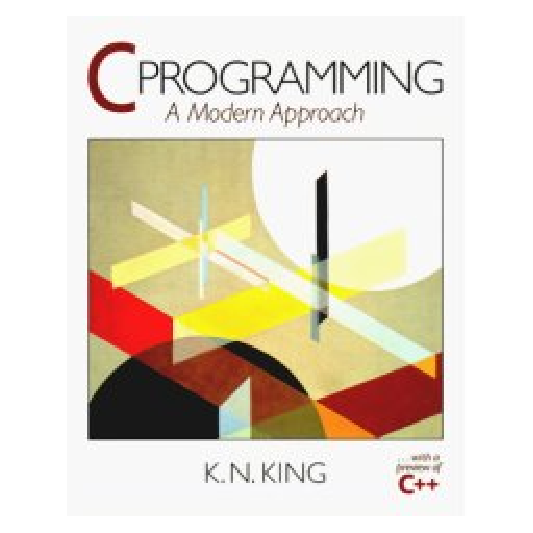
\includegraphics[width=\textwidth]{king}
\end{column}
\begin{column}{8cm}
\emph{C Programming A Modern Approach}
Norton \& Company. A well paced introduction to the C programming language with some introductory material to C++ too.
\end{column}
\end{columns}
\end{block}
\begin{block}<+->{\emph{Numerical Recipes in C++}}
\begin{columns}
\begin{column}{1.5cm}
\includegraphics[width=\textwidth]<2>{nr3rd}
\end{column}
\begin{column}{8cm}
By Press, Teukolsky, Vetterling \& Flannery, {\bf Third Edition}, CUP.
A C++ only, heavily revised edition of the text. If you want to perform scientific computations in C++ rather than C, I would recommend this. More information at:
\url{http://www.nr.com}
\end{column}
\end{columns}
\end{block}
\end{frame}

\begin{frame}
\frametitle{Building a C Program}
\begin{itemize}
\item To \emph{build} an executable from source, we carry out the following
three steps:
\begin{columns}
\begin{column}{3.1cm}
\begin{block}<+->{Edit Source}
Use a text editor to create a {\tt .c} file.
\end{block}
\end{column}
\begin{column}{3.8cm}
\begin{block}<+->{Compile}
With a C compiler, this creates \emph{object file(s)}.
\end{block}
\end{column}
\end{columns}
\begin{columns}
\begin{column}{3.8cm}
\begin{block}<+->{Link}
Combine the object files together into an \emph{executable}.
\end{block}
\end{column}
\end{columns}
\vspace{0.2in}
\item These steps are can be automated by \emph{Integrated Development Environments}
(IDEs).
\end{itemize}
\end{frame}

\ifhandout
\begin{frame}[fragile]
\frametitle{The Traditional Way to Start}
\begin{semiverbatim}
\kr\kl\kw{#include} \kt{<stdio.h>}
\kl
\kl\kw{int} main(\kw{void})
\kl\{
\kl   printf(\kt{"Hello World!\\n"});
\kl   \kw{return} 0;
\kl\}
\end{semiverbatim}

\begin{block}{The ``Hello World'' Program}
A traditional first program started by Ritchie. This is one of the smallest possible C programs that demonstrates some functionality (printing to screen).
\end{block}


\begin{block}{Line 1}
A \emph{pre-processor directive} (it begins with a {\tt \#}) advertising extra routines to the compiler.
\end{block}
\end{frame}

\begin{frame}
\begin{block}{Line 2}
An empty line, or equivalently, a line consisting solely of \emph{whitespace}. This is ignored by the compiler but makes the source code more readable.\end{block}

\begin{block}{Line 3}
A \emph{function declaration}, defining our {\tt main} function. The
{\tt main} function is where our program starts and is known as an
\emph{entry point}. Our main function takes \emph{no parameters} (\kw{\tt void}) and \emph{returns} an integer (\kw{\tt int}).
\end{block}

\begin{block}{Line 4}
\emph{Opening brace}, all statements enclosed between the braces {\tt\{}, {\tt\}} belong to the {\tt main} function.
\end{block}

\end{frame}

\begin{frame}
\begin{block}{Line 5}
A \emph{statement}; the \kw{\tt printf} (print formatted) function is called with the argument \kt{\tt "Hello World!$\backslash$n"}. This prints:\\
{\tt Hello World!}\\
to \emph{standard output} (usually a text console).
\end{block}

\begin{block}{Line 6}
A \emph{return statement}, we exit {\tt main} with a return code of 0. The system interprets 0 as ``success''.
\end{block}


\begin{block}{Line 7}
A \emph{closing brace}, everything after this line does not belong to
{\tt main}.
\end{block}

\end{frame}

\else
\begin{frame}[fragile]
\frametitle{The Traditional Way to Start}
\begin{semiverbatim}
\alert<2>{\kr\kl\kw{#include} \kt{<stdio.h>}}
\alert<3>{\kl}
\alert<4>{\kl\kw{int} main(\kw{void})}
\alert<5>{\kl\{}
\alert<6>{\kl   printf(\kt{"Hello World!\\n"});}
\alert<7>{\kl   \kw{return} 0;}
\alert<8>{\kl\}}
\end{semiverbatim}

\only<1>{\begin{block}{The ``Hello World'' Program}
A traditional first program started by Ritchie. This is one of the smallest possible C programs that demonstrates some functionality (printing to screen).
\end{block}
}

\only<2>{\begin{block}{Line 1}
A \emph{pre-processor directive} (it begins with a {\tt \#}) advertising extra routines to the compiler.
\end{block}}

\only<3>{\begin{block}{Line 2}
An empty line, or equivalently, a line consisting solely of \emph{whitespace}. This is ignored by the compiler but makes the source code more readable.\end{block}
}

\only<4>{\begin{block}{Line 3}
A \emph{function declaration}, defining our {\tt main} function. The
{\tt main} function is where our program starts and is known as an
\emph{entry point}. Our main function takes \emph{no parameters} (\kw{\tt void}) and \emph{returns} an integer (\kw{\tt int}).
\end{block}
}

\only<5>{\begin{block}{Line 4}
\emph{Opening brace}, all statements enclosed between the braces {\tt\{}, {\tt\}} belong to the {\tt main} function.
\end{block}
}

\only<6>{\begin{block}{Line 5}
A \emph{statement}; the \kw{\tt printf} (print formatted) function is called with the argument \kt{\tt "Hello World!$\backslash$n"}. This prints:\\
{\tt Hello World!}\\
to \emph{standard output} (usually a text console).
\end{block}
}

\only<7>{\begin{block}{Line 6}
A \emph{return statement}, we exit {\tt main} with a return code of 0. The system interprets 0 as ``success''.
\end{block}
}

\only<8>{\begin{block}{Line 7}
A \emph{closing brace}, everything after this line does not belong to
{\tt main}.
\end{block}
}

\vspace{10in}
%\vfill
\end{frame}
\fi

\ifhandout
\begin{frame}[fragile]
\frametitle {Another C Program - What does this do?}
\begin{semiverbatim}
\kr\kl\kw{#include} \kt{<stdio.h>}
\kl
\kl\kw{int} main(\kw{void})
\kl\{
\kl   \kw{int} low=-40, high=140, step=5, f, c;
\kl   c = low;
\kl   \kw{while} (c <= high)
\kl   \{
\kl      f = 32+9*c/5;
\kl      printf(\kt{"%6d \\t %6d\\n"}, c, f);
\kl      c = c + step;
\kl   \}
\kl   \kw{return} 0;
\kl\}
\end{semiverbatim}

\end{frame}

\begin{frame}
\begin{block}{Lines 1, 2, 3 \& 4}
Identical meaning as in the previous program.
\end{block}

\begin{block}{Line 5}
\emph{Local variable declarations}; the integers {\tt low}, {\tt high},
{\tt step}, {\tt f} and {\tt c} are declared. These are local to {\tt main}.
The variables {\tt low}, {\tt high} and {\tt step} are \emph{initialised}
with the values; whilst {\tt f} and {\tt c} are \emph{undefined}.
\end{block}
 
\begin{block}{Line 6}
The local variable {\tt c} is \emph{assigned} the value of
{\tt low}.
\end{block}

\begin{block}{Lines 7, 8 \& 12}
A \emph{while} loop is defined. For as long as the variable {\tt c} is less than or equal to {\tt high}, the code between the braces on lines 8 and 12 is executed.
\end{block}

\end{frame}

\begin{frame}
\begin{block}{Line 9}
The local variable {\tt f} is assigned a value from the integer arithmetic expression involving {\tt c}.
\end{block}

\begin{block}{Line 10}
The variables {\tt c} and {\tt f} are printed to standard out, each six characters
wide, separated by a tab and two spaces.
\end{block}

\begin{block}{Line 11}
The local variable {\tt c} is incremented by {\tt step}.
\end{block}

\begin{block}{Lines 13 \& 14}
Have an identical meaning as in the last program.
\end{block}

\end{frame}


\else
\begin{frame}[fragile]
\frametitle {Another C Program - What does this do?}
\begin{semiverbatim}
\only<1-4>{\alert<2>{\kr\kl\kw{#include} \kt{<stdio.h>}}
\alert<2>{\kl}
\alert<2>{\kl\kw{int} main(\kw{void})}
\alert<2>{\kl\{}
\alert<3>{\kl   \kw{int} low=-40, high=140, step=5, f, c;}
\alert<4>{\kl   c = low;}}
\only<1,5->{\alert<5>{\krr{7}\kl   \kw{while} (c <= high)}
\alert<5>{\kl   \{}
\alert<6>{\kl      f = 32+9*c/5;}
\alert<7>{\kl      printf(\kt{"%6d \\t %6d\\n"}, c, f);}
\alert<8>{\kl      c = c + step;}
\alert<5>{\kl   \}}
\alert<9>{\kl   \kw{return} 0;}
\alert<9>{\kl\}}}
\end{semiverbatim}

\only<2>{\begin{block}{Lines 1, 2, 3 \& 4}
Identical meaning as in the previous program.
\end{block}}
 
\only<3>{\begin{block}{Line 5}
\emph{Local variable declarations}; the integers {\tt low}, {\tt high},
{\tt step}, {\tt f} and {\tt c} are declared. These are local to {\tt main}.
The variables {\tt low}, {\tt high} and {\tt step} are \emph{initialised}
with the values; whilst {\tt f} and {\tt c} are \emph{undefined}.
\end{block}}
 
\only<4>{\begin{block}{Line 6}
The local variable {\tt c} is \emph{assigned} the value of
{\tt low}.
\end{block}}

\only<5>{\begin{block}{Lines 7, 8 \& 12}
A \emph{while} loop is defined. For as long as the variable {\tt c} is less than or equal to {\tt high}, the code between the braces on lines 8 and 12 is executed.
\end{block}}

\only<6>{\begin{block}{Line 9}
The local variable {\tt f} is assigned a value from the integer arithmetic expression involving {\tt c}.
\end{block}}

\only<7>{\begin{block}{Line 10}
The variables {\tt c} and {\tt f} are printed to standard out, each six characters
wide, separated by a tab and two spaces.
\end{block}}

\only<8>{\begin{block}{Line 11}
The local variable {\tt c} is incremented by {\tt step}.
\end{block}}

\only<9>{\begin{block}{Lines 13 \& 14}
Have an identical meaning as in the last program.
\end{block}}
\vspace{10in}
\end{frame}
\fi

%\subsection{Formatted Output}

% \begin{frame}
% \frametitle{{\tt printf} - declared in \kt{\tt <stdio.h>}}
% As seen in the examples, the {\tt printf} function can be used to print out variables. The function \emph{prototype} takes the form:
% \begin{center}
% {\tt \alert<4>{\kw{int}} printf(\alert<2>{\kw{char} * formatString}, \alert<3>{...})}
% \end{center}
% \begin{block}<2>{{\tt formatString}}
% The first argument of {\tt printf} is the \emph{format string}, this specifies how many variables need printing out, how they are to be printed, and in what order.
% \end{block}
% \begin{block}<3>{{\tt ...}}
% This is C shorthand for \emph{variable number of arguments}.
% \end{block}
% 
% \begin{block}<4>{Return value: {\tt int}}
% {\tt printf} returns the number of characters printed.
% \end{block}
% \end{frame}
% 

\begin{frame}
\frametitle{{\tt printf} - declared in \kt{\tt <stdio.h>}}
We call {\tt printf} as follows:
\begin{center}
\tt printf(formatString, var1, var2, $\ldots$, varN);
\end{center}
where,
\begin{block}{\tt formatString}
The format string tells {\tt printf} how many variables need printing. A format string can contain \emph{format specifiers}, these tell {\tt printf} exactly how to print out each variable, some examples:
\begin{tabular}{l l}
\tt\kt{"\%6d"} & print out an integer (6 characters wide).\\
\tt\kt{"\%g"} & print out a floating point number.
\end{tabular}
\end{block}
\begin{block}{\tt var1, ...}
{\tt printf} accepts a variable list of arguments, which can be of different type. Care must be taken to match {\tt formatString} with the variables.
\end{block}
\end{frame}

\begin{frame}
\frametitle{Special Characters}
\begin{itemize}
\item The backslash {\tt $\backslash$} character in C has a special meaning, it is known as the \emph{escape character}.
\item We combine the escape character with other characters, to form an \emph{escape sequence}, here are some examples:
\begin{center}
\begin{tabular}{l r}
\begin{tabular}{r l}
{\tt $\backslash$n} & New line\\
{\tt $\backslash$t} & Tab\\
{\tt $\backslash$b} & Backspace\\
{\tt $\backslash$r} & Carriage return\\
{\tt $\backslash$a} & Bell
\end{tabular}&
\begin{tabular}{r l}
{\tt $\backslash$f} & Form feed (new page)\\
{\tt $\backslash\backslash$} & $\backslash$\\
{\tt $\backslash$"} & "\\
{\tt $\backslash$'} & '
\end{tabular}
\end{tabular}
\end{center}
\end{itemize}
\end{frame}

%\subsection{Numbers}
\begin{frame}[fragile]
\frametitle{Numbers in C - 2 General Types}
\begin{itemize}
\item \emph{Integers} - \kw{{\tt short}, {\tt unsigned short}, {\tt int}, {\tt unsigned int}, {\tt long}, {\tt unsigned long}, {\tt long long}, {\tt unsigned long long}}. Integer types in C can be thought of as rings of different sizes (i.e. hours on a clock face). Most importantly remember that division is not necessarily the inverse of multiplication.
\item \emph{Floats} - \kw{{\tt float}, {\tt double}, {\tt long double}}.
These are \emph{NOT} the same as $\mathbb{R}$ (associativity, and even commutativity not guaranteed, multiplicative inverses don't always exist). Programming
floats well for numerical problems with large/small numbers is an art form.
\end{itemize}
\end{frame}

\begin{frame}
\frametitle{Integer Types - For my 32 bit Windows Box}
\resizebox{\textwidth}{!}{
\rowcolors[]{1}{blue!20}{blue!10}
\begin{tabular}{r !{\vrule} r l}
\bf Type&\bf Min&\bf Max\\
\hline
short&-32768&32767\\
unsigned short&0&65535\\
int&-2147483648&2147483647\\
unsigned int&0&4294967295\\
long&-2147483648&2147483647\\
unsigned long&0&4294967295\\
long long&-9223372036854775808&9223372036854775807\\
unsigned long long&0&18446744073709551615
\end{tabular}}
\vspace{2ex}\\
For example, here are two bit patterns for \kw{\tt short}:
\begin{center}
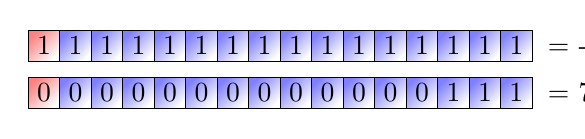
\begin{tikzpicture}[]
\shadedraw [top color=red!50,shading angle=45] (0,0) rectangle +(0.4,0.4);
\node at (0.2,0.2) {0};
\foreach \x in {0.4, 0.8, ..., 6.4}
   \shadedraw [top color=blue!50,shading angle=45] (\x,0) rectangle +(0.4,0.4);
\foreach \x in {0.6, 1.0, ..., 5.0}
   \node at (\x, 0.2){0};
\foreach \x in {5.4, 5.8, 6.2}
   \node at (\x, 0.2){1};   
\node at (6.6, 0.2){\rlap{= 7}};

\shadedraw [top color=red!50, shading angle=45] (0,0.6) rectangle +(0.4,0.4);
\foreach \x in {0.4, 0.8, ..., 6.4}
   \shadedraw [top color=blue!50, shading angle=45] (\x,0.6) rectangle +(0.4,0.4);
\foreach \x in {0.2, 0.6, ..., 6.6}
   \node at (\x, 0.8){1};
\node at (6.6, 0.8){\rlap{= -1}};
\end{tikzpicture}
\end{center}
(for more information see \kt{\tt <limits.h>})
\end{frame}


\begin{frame}
\frametitle{Integer Types(2)}
\begin{itemize}
\item Two main subtypes \emph{signed} and \emph{unsigned}. Signed types use a sign bit.
\item For signed types we, usually, have:
\begin{itemize}
\item minimum value: $-2^{\textrm{size}-1}$
\item maximum value: $2^{\textrm{size}-1}-1$
\end{itemize}
\item For unsigned types we have:
\begin{itemize}
\item minimum value: $0$
\item maximum value: $2^{\textrm{size}}-1$
\end{itemize}
\item \kw{\tt short} is often used to conserve memory.
\item \kw{\tt int} represents the \emph{native} CPU integer type so is used for speed. (If in doubt use \kw{\tt int}).
\item \kw{\tt long} and \kw{\tt long long} are used to maintain accuracy.
\end{itemize}
\end{frame}

\begin{frame}
\frametitle{Integer Arithmetic}

\begin{block}{Base Operators}
The four usual operators are defined $+$, $-$, {\tt *} and $/$.
\end{block}

\begin{block}{Ring arithmetic}
Division is not always the reverse of multiplication:\\
{\tt 1/2=0,  0*2=0.}\\
Also, any result of a computation must lie within the ring, any number outside the range of the current data type will ``wrap'' around. (i.e. 11am + 3 hours gives 2pm).
\end{block}

\begin{block}{Remainder Operator}
The remainder operator {\tt\%} is unique to integer types, it acts as expected:
{\tt7\%2 = 1}.
\end{block}
\end{frame}

\begin{frame}
\frametitle{Floating Point Numbers (IEEE 754 Standard)}
On my machine, a \kw{\tt float} (single precision) looks like:\\
\begin{center}
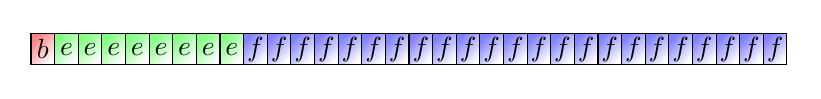
\begin{tikzpicture}[]
\shadedraw [top color=red!50,shading angle=45] (0,0) rectangle +(0.3,0.4);
\node at (0.15,0.2) {$b$};
\foreach \x in {0.3, 0.6, ..., 2.7}
   \shadedraw [top color=green!50,shading angle=45] (\x,0) rectangle +(0.3,0.4);

\foreach \x in {0.45, 0.75, ..., 2.85}
   \node at (\x,0.2) {$e$};
   
\foreach \x in {2.7, 3.0, ..., 9.6}
   \shadedraw [top color=blue!50,shading angle=45] (\x,0) rectangle +(0.3,0.4);
   
\foreach \x in {2.85, 3.15, ..., 9.45}   
   \node at (\x,0.2) {$f$};
\end{tikzpicture}
\end{center}
It consists of three parts, the \textcolor{red}{\emph{sign bit}$(b)$}, the \textcolor{green}{\emph{biased exponent}$(e)$} and the \textcolor{blue}{\emph{fraction}$(f)$}.
We break down a number $x$:
$$x^{\textrm{float}} = \textcolor{red}{(-1)^b} \times 
\textcolor{green}{2^{e-127}} \times \textcolor{blue}{\left(1+f\times2^{-23}\right)},
\begin{array}{c}
0 < e < 255\\0 \leq f \leq 2^{23}-1
\end{array},$$
We have three special numbers, {\tt -Inf} ($-\infty$), {\tt Inf} ($\infty$) and {\tt NaN} (Not a Number).

For \kw{\tt double} (double precision) we have:
$$x^{\textrm{double}} = (-1)^b\times 2^{e-1023}\times\left(1+f\times2^{-52}\right),
\begin{array}{c}
0 < e < 2047\\0 \leq f \leq 2^{52}-1
\end{array}.$$
\end{frame}

\begin{frame}
\frametitle{Floating Point}
\begin{block}{Base Operators}
As with integers, we have $+$, $-$, {\tt *} and $/$.
\end{block}

\begin{block}{Floating point code}
\begin{itemize}
\item It looks like integer code but with a decimal point suffix.
\item Scientific notation is achieved with {\tt e}:\\
{\tt \kw{double} speedofLight = 2.997e8;} ($2.997 \times 10^8$)
\end{itemize}
\end{block}

\begin{block}{Float Arithmetic}
\begin{itemize}
\item Division is not always the reverse of multiplication.
\item Operators may not be commutative!
$$ A + B + C \neq A + C + B \qquad \mathrm{(sometimes)}$$
\end{itemize}
\end{block}

\end{frame}


\begin{frame}
\frametitle{The {\tt pow(x, y)} function (declared in \kt{\tt <math.h>})}
\begin{block}{Exponentiation}
There is no exponentiation operator (e.g. $\wedge$, {\tt **}) in C. Instead we have the following:
$$x^y = \mathrm{\tt pow(x,y)}$$
This assumes $x$ and $y$ are of type \kw{\tt double}.
\end{block}

\begin{alertblock}{Beware}
The {\tt pow} function is often implemented as:
\begin{center}{\tt exp(y*ln(x))}\end{center}
For whole integer powers (i.e. $x^2$), one should perform the multiplication explicitly ({\tt x*x}).
\end{alertblock}
\end{frame}

\begin{frame}
\frametitle{More Mathematical Functions in \kt{\tt <math.h>}}
\begin{itemize}
\item Maths functions come with the \emph{ANSI Standard C Library}, which contains many maths functions. To use them we need a:
{\tt \kw{\#include} \kt{<math.h>}}
\item Here some example functions:
\begin{tabular}{l l l l}
\tt sin(x)&\tt asin(x) & \tt sinh(x) & \tt exp(x)\\
\tt cos(x)&\tt acos(x) & \tt cosh(x) & \tt log(x)\\
\tt tan(x)&\tt atan(x) & \tt tanh(x) & \tt log10(x)\\
\tt sqrt(x)&\tt atan2(x,y)&\tt pow(x,y) & \tt fabs(x)
\end{tabular}\\
\vspace{1ex}
(all the trigonometric functions use radians!)
\end{itemize}
\end{frame}

\begin{frame}
\frametitle{Commenting C Programs}
There are two ways of commenting files in C.

\begin{block}{Traditional Way}
Anything between {\tt /*} and {\tt */} is a comment, i.e.\\
\kc{\tt /* Hello World! */}\\
and,\\
{\tt \kc{/* This function is used to compute the} }\\
{\tt \kc{roots of a quadratic equation */}}
\end{block}

\begin{block}{C++ Style}
These are single line only, anything after {\tt //} is a comment, i.e.\\
{\tt \kw{int} c = 3; \kc{// set c to 3}}
\end{block}

\begin{alertblock}{}
Technically, C++ style comments aren't in the C standard. (But they are
ubiquitous to C code anyway).
\end{alertblock}
\end{frame}

\begin{frame}
\frametitle{Variable Names}
\begin{block}{From K\&R}
``... Is a sequence of letters and digits. The first character must be a letter; the underscore \_ counts as a letter. Upper and lower case letters are different.''
\end{block}

\begin{itemize}
\item Punctuation or any other symbols are not allowed in variable names.
\item The modern C standard discourages the use of an underscore as the first character of a variable name.
\end{itemize}
\end{frame}

\begin{frame}
\frametitle{Simple Logical Expressions}
\begin{itemize}
\item Are used to carry out branches ({\tt \kw{if}} statement) and loops (such as {\tt \kw{for}}, and {\tt \kw{while}}).
\item Evaluate to either \emph{true} (non-zero \kw{\tt int}) or \emph{false} (zero).
\end{itemize}

\begin{block}{Logical Operators}
\begin{center}
\begin{tabular}{l c l l}
\tt x &\tt>&\tt  y& is {\tt x} greater than {\tt y}?\\
\tt x &\tt>=&\tt y& is {\tt x} greater than or equal to {\tt y}?\\
\tt x &\tt<&\tt  y& is {\tt x} less than {\tt y}?\\
\tt x &\tt<=&\tt y& is {\tt x} less than or equal to {\tt y}?\\
\alert{\tt x }&\tt\alert{==}&\alert{\tt y}&\alert{is {\tt x} equal to {\tt y}?}\\
\tt x &\tt!=&\tt y& is {\tt x} different to {\tt y}?
\end{tabular}
\end{center}
\end{block}
\end{frame}

\begin{frame}
\frametitle{Compound Logical Expressions}
We can create compound logical expressions using the following operators:
\begin{itemize}
 \item {\tt ||} is a \emph{logical or}. {\tt le1 || le2} returns false if both {\tt le1} and {\tt le2} are false and true otherwise.
 \item {\tt \&\&} is a \emph{logical and}. {\tt le1 \&\& le2} returns true if and only if both {\tt le1} and {\tt le2} are true.
 \item {\tt !} is a \emph{logical not}. {\tt !le1} returns the opposite of {\tt le1}.
\end{itemize}
Here are two identical examples:
\begin{itemize}
\item \tt (x < 100) \&\& (x\%2 == 0)\\
\item \tt (x < 100) \&\& !(x\%2)
\end{itemize}
\end{frame}

\begin{frame}[fragile]
\frametitle{Flow Control - {\tt if}}
Executes block(s) of code depending on the evaluation of a logical expression.
\begin{block}{Simple {\tt if}}
\begin{center}{\tt \kw{if} (}\emph{logical expression}{\tt ) \{}\emph{statements}{\tt ;\}}\end{center}
\end{block}

\begin{block}{{\tt if}, {\tt else if}, {\tt else}}
\begin{semiverbatim}
   \kw{if} (\emph{logical expression})
      \{\emph{statements};\}
   \kw{else if} (\emph{logical expression})
      \{\emph{statements};\}
   \kw{else if} (\emph{logical expression})
      \{\emph{statements};\}
   \kw{else}
      \{\emph{statements};\}
\end{semiverbatim}
\end{block}
\end{frame}

\begin{frame}[fragile]
\frametitle{Flow Control - {\tt while}}
A \kw{\tt while} loop is used to repeatedly execute code as long as a logical expression is true.

\begin{block}{Structure}
\begin{semiverbatim}
   \kw{while} (\emph{logical expression})
      \{ \emph{statements} ;\}
\end{semiverbatim}
\end{block}
\begin{itemize}
\item If \emph{logical expression} is false, then the \emph{statements} are never executed.
\end{itemize}
\end{frame}

\begin{frame}[fragile]
\frametitle{Flow Control - {\tt do \{\} while ()}}
We place the \emph{logical expression} after the \emph{statements} giving us:
\begin{block}{Structure}
\begin{semiverbatim}
   \kw{do} \{\emph{statements};\}
   \kw{while} (\emph{logical expression})
\end{semiverbatim}
\end{block}
\begin{itemize}
\item The \emph{statements} are executed at least once.
\end{itemize}
\begin{exampleblock}{{\tt do while} or {\tt while}?}
Generally I prefer {\tt \kw{while}} over {\tt \kw{do while}}, as it forces me to initialise variables properly.
\end{exampleblock}
\end{frame}

\begin{frame}[fragile]
\frametitle{Flow Control - {\tt for} loop}
\begin{block}{}
\begin{semiverbatim}
   \kw{for} ( \emph{start expression} ;
         \emph{logical expression} ;
         \emph{step expression})
         \{ \emph{statements} ;\}
\end{semiverbatim}
\end{block}
\begin{itemize}
\item Print out ten numbers:
\begin{semiverbatim}
   \tt\kw{for} (x=0; x < 10; x = x + 1)
      printf(\kt{"x = %d\\n"}, x);
\end{semiverbatim}
\item Keep looping indefinitely (printing out dots)
\begin{semiverbatim}
   \kw{for} (;;) printf(\kt{"."});
\end{semiverbatim}
\end{itemize}
\end{frame}

\begin{frame}[fragile]
\frametitle{Flow Control - \tt switch - case}
We can selectively execute code based on a value, using the following:
\begin{block}{}
\begin{semiverbatim}
   \kw{switch} (\emph{integer\_statement}) \{
   \kw{case} \emph{integer\_value1}: \emph{statements1}; \kw{break};
   \kw{case} \emph{integer\_value2}: \emph{statements2}; \kw{break};
   \kw{case} \emph{integer\_value3}:
   \kw{case} \emph{integer\_value4}: \emph{statements3}; \kw{break};   
   \kw{default}: \emph{statements4}; \kw{break};\}
\end{semiverbatim}
\end{block}
\begin{itemize}
\item Execution starts at either one of the \kw{\tt case}'s or at \kw{\tt default}.
\item Execution stops at the end {\tt\}} or at \kw{\tt break}.
\item \kw{\tt case}, \kw{\tt default} and \kw{\tt break} are optional.
\end{itemize}
\end{frame}

\begin{frame}{Some Loop Control Features}
Execution of code inside a loop (\kw{\tt do}, \kw{\tt while}, \kw{\tt for})
can be manipulated by the following statements.
\begin{block}{\tt break;}
Break out of the current loop. Any statements in the loop following the \kw{\tt break} are ignored and the loop condition automatically evaluates to false, ending the loop.
\end{block}
\begin{block}{\tt continue;}
Jump to the end of the current loop (effectively ignoring everything below the \kw{\tt continue} statement. Whether or not the loop continues executing depends on the loop condition.
\end{block}
\end{frame}

\begin{frame}{{\tt scanf()} - Reading Data from Standard Input}
For two variables {\tt A} and {\tt B}, both of type \kw{\tt double}, we use:
\begin{center}
\tt scanf(\kt{"\%lf \%lf"}, \&A, \&B);
\end{center}
\begin{itemize}
\item where the {\tt\%} represent \emph{format specifiers}
\begin{block}{Format Specifiers}
Consist of a {\tt\%}, a numerical width specification and a field code:
\resizebox{\textwidth}{!}{
\begin{tabular}{c c}
\begin{tabular}{l l}
\tt d& \kw{\tt int}\\
\tt u& \kw{\tt unsigned int}\\
\tt f& \kw{\tt float} (fixed form)\\
\tt e& \kw{\tt float} (exponential form)
\end{tabular}&
\begin{tabular}{l l}
\tt g & \kw{\tt float} (general form)\\
\tt lf & \kw{\tt double} (fixed form)\\
\tt le & \kw{\tt double} (exponential form)\\
\tt lg & \kw{\tt double} (general form)
\end{tabular}
\end{tabular}}
\end{block}
\item and the {\tt\&} represents the \emph{address} of the variable in memory. This is known as a \emph{pointer reference operator}.
\end{itemize}
\end{frame}

\begin{frame}
\frametitle{Why the {\tt \&A} in {\tt scanf()}?}
\begin{itemize}
\item Functions in C can return only one value.
\item Sometimes we want more than one value to change.
\item If we tell {\tt scanf} \emph{where} the variables are in memory,
{\tt scanf} can change them itself.
\end{itemize}

\begin{alertblock}{}
The ability to manipulate memory directly is what makes C so powerful.
(and potentially dangerous).
\end{alertblock}
\end{frame}

{
%\setbeamercolor{stucture}{bg=red}
\setbeamercolor{frametitle}{bg=red}
\begin{frame}[fragile]
\frametitle{Pointers}
A \emph{pointer} is a variable that stores a memory location, they are declared as follows:
\begin{center}
\tt \kw{double} * ptrA;
\end{center}

\begin{block}{{\tt \&} - Pointer reference operator}
Returns the memory address (pointer to) of a variable.
\begin{semiverbatim}
   \kw{double} * ptrA = \&A;   \kc{// ptrA points to A}
\end{semiverbatim}
\end{block}

\begin{block}{{\tt *} - Pointer de-reference operator}
Converts a memory address to a variable:
\begin{semiverbatim}
   * ptrA  = 1.234;      \kc{// A is now 1.234}
\end{semiverbatim}
\end{block}

\end{frame}
}

\begin{frame}
\frametitle{Defining Functions}
The C language only provides essential functionality, meaning a lot of functions need to be written yourself. Here are a few general rules for functions:

\begin{itemize}
\item Functions cannot define other functions within them.
\item An optional single value can be returned.
\item All arguments to a functions are passed by value and remain unaffected by the function.
\item Passing pointers to functions allows them to ``return'' multiple variables.
\end{itemize}
\end{frame}

\begin{frame}
\frametitle{An Example: Quadratic Equation Solver}
As a worked example we write a function to solve the quadratic equation:
$$ A x^2 + B x + C=0 \qquad A,B,C\in\mathbb{R}$$
Our quadratic solver will:
\begin{itemize}
\item Take the three doubles {\tt A}, {\tt B} and {\tt C} as arguments.
\item Solve the quadratic and return an \kw{\tt int} signifying to the caller the type of answer available:
\begin{tabular}{l l}
-1&{\tt A} = 0, we have a linear equation.\\
0&There are two distinct real roots.\\
1&We have a pair of complex conjugate roots.\\
2&Both roots are real and identical.
\end{tabular}
\end{itemize}
\end{frame}

\begin{frame}[fragile]
\frametitle{The Code}
One possible function prototype is:
\begin{semiverbatim}
\kw{int} quad_roots (\kw{double} A, \kw{double} B, \kw{double} C,
                \kw{double} * r1, \kw{double} * r2);
\end{semiverbatim}
\begin{itemize}
\item The variables {\tt A}, {\tt B} and {\tt C} are unchanged by {\tt quad\_roots}.
\item We need to return two doubles (the roots of the equation), thus we take in pointers {\tt \kw{double} *r1} and {\tt \kw{double} *r2}.
\item C90 does not allow for complex number types (C99 does support them), so we have to think a little bit about the complex number case.
\end{itemize}
\end{frame}

\begin{frame}[fragile]
\frametitle{Code Snippet for Calling {\tt quad\_roots}}
\begin{semiverbatim}
...
\kw{int} main()
\{
   \kw{double} A, B, C, root1, root2;
   \kw{int} quad_case;   
   ...   
   quad_case = quad_roots(A, B, C, &root1,
                          &root2);
                          
   \kw{switch}(quad_case)
   \{
   \kw{case} -1: \emph{linear equation}
\end{semiverbatim}
\end{frame}

\begin{frame}[fragile]
\frametitle{Code Snippet for {\tt quad\_roots}}
\begin{semiverbatim}
\kw{int} quad_roots(\kw{double} A, \kw{double} B, \kw{double} C,
               \kw{double} * r1, \kw{double} *r2)
\{
   \kw{double} d;
   
   \kc{/* linear case */}
   if (A == 0.0)
   \{
      *r1 = -C/B;
      \kw{return} -1;
   \}
          
   \kc{/* compute the discriminant */}
   d = B*B-4.0*A*C;
\end{semiverbatim}
\end{frame}

\begin{frame}[fragile]
\frametitle{Declarations vs Definitions}
\begin{block}{Function Declarations}
These tell the compiler about the \emph{existence} of a function, which then
allows us to call it. A declaration ends with a {\tt ;}.
\begin{semiverbatim}
\kw{int} quad_roots (\kw{double} A, \kw{double} B, \kw{double} C,
                \kw{double} * r1, \kw{double} * r2);
\end{semiverbatim}
\end{block}

\begin{block}{Function Definitions}
The code making up the function is supplied to the compiler. A function can only be defined once. A definition contains braces {\tt \{} and {\tt \}}:
\begin{semiverbatim}
\kw{int} quad_roots (\kw{double} A, \kw{double} B, \kw{double} C,
                \kw{double} * r1, \kw{double} * r2)
\{...\}
\end{semiverbatim}
\end{block}
\end{frame}

% \begin{frame}
% \frametitle{Graphics}
% \tikzstyle{level 1}=[sibling angle=120]
% \tikzstyle{level 2}=[sibling angle=60]
% \tikzstyle{level 3}=[sibling angle=30]
% \tikzstyle{every node}=[fill]
% \tikzstyle{edge from parent}=[snake=expanding waves,segment length=1mm,segment angle=10,draw]
% \tikz [grow cyclic,shape=circle,very thick,level distance=10mm,cap=round]
% \node {} child [color=\A] foreach \A in {red,green,blue}
% { node {} child [color=\A!50!\B] foreach \B in {red,green,blue}
% { node {} child [color=\A!50!\B!50!\C] foreach \C in {black,gray,white}
% { node {} }
% }
% };
% \end{frame}
% 
% \begin{frame}
% \frametitle{More Graphics}
% \begin{columns}
% \begin{column}{4cm}
% \begin{tikzpicture}[edge from parent fork down]
% \tikzstyle{every node}=[fill=red!30,rounded corners]
% \tikzstyle{edge from parent}=[red,-o,thick,draw]
% \node {root}
% child {node {left}}
% child {node {right}
% child {node {child}}
% child {node {child}}
% };
% \end{tikzpicture}
% \end{column}
% \begin{column}{4cm}
% \begin{tikzpicture}
% [parent anchor=east,child anchor=west,grow=east]
% \tikzstyle{every node}=[ball color=red,circle,text=white]
% \tikzstyle{edge from parent}=[draw,dashed,thick,red]
% \node {root}
% child {node {left}}
% child {node {right}
% child {node {child}}
% child {node {child}}
% };
% \end{tikzpicture}
% \end{column}
% \end{columns}
% \end{frame}


\end{document}




